% Generated supplement source: scripts/build_paper.py fills {{VAL:...}} and {{TABLE:...}} and writes paper/supplement.tex.
\documentclass[10pt]{article}
\usepackage[margin=2cm]{geometry}
\usepackage{amsmath,amssymb}
\usepackage{graphicx}
\usepackage{booktabs}
\usepackage{longtable}
\usepackage{float}
\usepackage[hidelinks]{hyperref}
\usepackage{url}
\renewcommand{\thetable}{S\arabic{table}}
\renewcommand{\thefigure}{S\arabic{figure}}
\begin{document}
\begin{center}
{\large Supplementary material}\\[2pt]
{\normalsize A Lidar Benchmark for Desert Rover Traversability: Slip Face Detection, Hazard Layers and Route Planning from Coarse Elevation Models on Active Sand Dunes}
\end{center}

\section*{S1. Prediction log}
Every experiment of this benchmark was designed and given numeric predictions before it ran, and the predictions were committed to the repository (\url{docs/PREDICTIONS.md}) before any metric of that stage was computed. Stages 25 and 26 were the first version of the benchmark; stages 27 and 28 were registered after a blind review of that version and before any of their metrics were computed, when the results of stages 25 and 26 were known. Table~\ref{tab:log} copies every prediction verbatim with its recorded outcome: 31 hits and 12 misses out of 43 predictions. Three amendments were made before the affected results were known, each recorded in the log with its reason: the closed loop uses 20 pairs per site, a 300\,m crop margin and the radius and vehicle sensitivities on I30 only (compute budget); after a first tuning attempt was stopped because it would not finish, the nested tuning of boosting fits its inner folds on at most 150\,000 cells; and after a first closed loop run was stopped, with its outcomes unseen, each pair has a budget of 300 replans. Results decided after a run (for example the post hoc analyses of stages 25 and 26, and stages 29 and 30, the post hoc checks of the paper) are labelled as such in the log; the predictions of stages 29 and 30 were written before their runs but carry no confirmatory weight and are not counted above. Correction notes appended after a number audit (rounding of two outcomes and the scope of two others; no scoring changed) are in the log. The log lives in our own repository, not in a public registry, and the six windows had been used in earlier tests of the detector.

\begin{longtable}{@{}p{0.08\linewidth}p{0.42\linewidth}p{0.46\linewidth}@{}}
\caption{Prediction log of stages 25 to 30: every prediction as committed before its run (verbatim) and the outcome as recorded afterwards. Stages 29 (X29) and 30 (Y30) are post hoc and not counted in the tally.}\label{tab:log}\\
\toprule
ID & Prediction (before the run) & Outcome \\
\midrule
\endhead
B25-1 & On I30, GBM beats DET (paired interval excludes zero, GBM higher) at three or more of the six sites, and the macro mean AUC difference GBM minus DET lies between 0.00 and 0.12. & HIT. GBM beats DET at all six sites on I30 (paired block bootstrap interval above zero), macro mean AUC 0.806 against 0.741, difference 0.065 (\url{results/benchmark/detection/paired_differences.csv}, \url{macro.csv}). \\
B25-2 & On I30, the AUC point estimate of DET is higher than that of SLOPE at four or more of the six sites. & HIT (4 of 6). DET above SLOPE on I30 at White Sands (0.658 against 0.584), Great Sand Dunes (0.831 against 0.708), Algodones (0.761 against 0.691) and Little Sahara (0.637 against 0.533); below at Dumont (0.860 against 0.931) and Kelso (0.700 against 0.743). \\
B25-3 & On I30, no method reaches an AUC of 0.90 at more than two of the six sites. & HIT. On I30 only Dumont reaches 0.90 (SLOPE, TRI, ROUGH, BICUBIC, GBM and CNN 0.93 to 0.96); no method reaches 0.90 at any other site (highest: CNN 0.893 at Great Sand Dunes). \\
B25-4 & On I10, DET, GBM and CNN each reach an AUC of at least 0.93 at every site. & MISSED. GBM (0.937 to 0.985) and CNN (0.935 to 0.982) reach 0.93 everywhere on I10, DET does not at Little Sahara (0.908; elsewhere 0.953 to 0.973). \\
B25-5 & On I30, the macro mean AUC of BICUBIC exceeds that of SLOPE by at most 0.02. & MISSED, in the opposite direction to the prediction. BICUBIC exceeds SLOPE by 0.118 macro mean AUC on I30 (0.817 against 0.699) and is the best method on I30 by mean AUC, ahead of GBM (0.806), CNN (0.795) and DET (0.741): the steepest slope of the interpolated surface carries curvature information that the coarse slope lacks. \\
B25-6 & The macro mean AUC of DET on G30 is lower than on I30 by at least 0.03. & HIT. Macro mean AUC of DET 0.646 on G30 against 0.741 on I30 (difference 0.095). \\
B25-7 & On G30, every method has a macro mean AUC below 0.85. & HIT. On G30 the highest macro mean AUC is 0.727 (CNN), then GBM 0.722 and BICUBIC 0.697; at White Sands every unsupervised method is at chance (0.46 to 0.52). \\
B25-8 & On I30, DET-cal has a lower Brier score than DET at five or more of the six sites. & HIT (6 of 6). Brier score on I30, DET-cal against DET: Dumont 0.150 against 0.217, White Sands 0.221 against 0.254, Kelso 0.195 against 0.256, Great Sand Dunes 0.138 against 0.159, Algodones 0.144 against 0.179, Little Sahara 0.206 against 0.249. \\
B25-9 & On I30, the macro mean AUC of CNN lies within 0.05 of that of GBM. & HIT. CNN 0.795 against GBM 0.806 macro mean AUC on I30 (difference 0.011). \\
P26-1 & On I30, no hazard layer with either cautious policy raises pooled mission success above naive by more than 15 points. & MISSED, because of the oracle only. On I30 the ORACLE layer raised mission success from 6.2 \% (naive) to 59.0 \% (conservative) and 50.2 \% (risk weighted). Every layer a rover could actually compute stayed within 5 points of naive: the best was BICUBIC-cal with the risk weighted policy, 11.0 \% (plus 4.8 points, Holm corrected McNemar p 0.00002); DET 6.8 \% and 7.0 \%, GBM 6.2 \% and 7.2 \%, CNN 6.8 \% and 8.5 \% (\url{results/benchmark/planning/summary.csv}, \url{tests.csv}). \\
P26-2 & On I10, the conservative policy with DET has a pooled unsafe share at least 15 points lower than naive, significant after Holm correction. & MISSED. On I10 the conservative policy with DET is unsafe on 72.4 \% of routed pairs against 85.3 \% for naive (12.9 points lower, not 15); its mission success, 24.3 \% against 14.7 \%, is significantly higher (Holm corrected McNemar p below 0.0001). \\
P26-3 & On I30, the conservative policy with ORACLE has a pooled unsafe share at least 20 points lower than with DET. & HIT. On I30 the conservative policy is unsafe on 31.9 \% of routed pairs with ORACLE against 92.5 \% with DET. \\
P26-4 & ORACLE-5 has a pooled unsafe share of at most 5 \%. & HIT. ORACLE-5 routed all 600 pairs and none crossed a face patch (unsafe 0.0 \%, length 1.30 times the straight distance). \\
P26-5 & SHORTEST is unsafe on at least 60 \% of pairs, pooled. & HIT. SHORTEST is unsafe on 96.2 \% of pairs on the 30 m grid and 96.0 \% on the 10 m grid. \\
P26-6 & On G30, the pooled unsafe share of the conservative policy with DET is at least that on I30 minus 5 points. & HIT. The conservative policy with DET is unsafe on 94.4 \% of routed pairs on G30 against 92.5 \% on I30. \\
P26-7 & On I30, the pooled unsafe share of the conservative policy with GBM is at most 10 points lower than with DET. & MISSED. On I30 the conservative policy with GBM is unsafe on 67.3 \% of routed pairs against 92.5 \% with DET (25 points lower), but it routes only 18.8 \% of pairs against 91.2 \%, so its mission success is no higher (6.2 \% against 6.8 \%). \\
P26-8 & On I10, the mean length over straight distance of conservative routes with DET is at most 1.5. & HIT. Mean length over straight distance of conservative DET routes on I10: 1.17. \\
D27-1 & On I30 against L-ANY, BICUBIC has the highest or tied highest macro mean AUC among DET, SLOPE, TRI, ROUGH, BICUBIC, GBM and CNN (tied: within 0.01). & HIT. On I30 against L-ANY interpolation has the highest macro mean AUC of the seven (0.817; GBM 0.810, CNN 0.800, ROUGH 0.770, TRI 0.764, DET 0.740, SLOPE 0.689; \url{results/benchmark/stage27/A_macro.csv}). Part G later found a network trained four times longer at 0.838, which is not one of the seven. \\
D27-2 & On I30, the macro mean AUC against L-ANY is lower than against L-CELL for at least five of the seven stage 25 methods. & MISSED. Lower against L-ANY for 3 of 7 methods (DET 0.740 against 0.741, SLOPE 0.689 against 0.699, BICUBIC 0.8165 against 0.8167) and higher for TRI, ROUGH, GBM and CNN; every difference is 0.01 or less, so the label change hardly matters on I30. \\
D27-3 & I10 to 30 (maximum of the 10 m scores) beats the same method on I30 against L-ANY by at least 0.05 macro mean AUC for BICUBIC and GBM. & HIT. The maximum of the nine 10 m scores, scored on I30 L-ANY, beats the 30 m surface by 0.141 for BICUBIC (0.957 against 0.817) and 0.149 for GBM (0.959 against 0.810). \\
D27-4 & Resolution sweep: the macro mean AUC of BICUBIC and GBM falls monotonically from 2 to 60 m (one inversion of at most 0.01 allowed per method). & HIT. BICUBIC 0.999, 0.993, 0.968, 0.934, 0.895, 0.817 and 0.693 and GBM 0.999, 0.992, 0.968, 0.935, 0.895, 0.810 and 0.673 at 2, 5, 10, 15, 20, 30 and 60 m, with no inversion (\url{results/benchmark/stage27/C_macro.csv}). \\
D27-5 & Resolution sweep: at 2 m, SLOPE reaches a macro mean AUC of at least 0.95; at 60 m, no method exceeds 0.80. & HIT. SLOPE reaches 0.996 at 2 m; at 60 m the best method is BICUBIC at 0.693. \\
D27-6 & Scaling: pooled patch recall of GBM is at least 0.8 for L/d of 2 or more and at most 0.5 for L/d below 0.5, at every posting where both bins hold at least 50 patches. & MISSED. For L/d below 0.5 the recall of GBM is 0.87 at 10 m, 0.76 at 15 m, 0.68 at 20 m, 0.60 at 30 m and 0.46 at 60 m (above 0.5 except at 60 m), and for L/d of 2 or more it is at least 0.91 from 10 to 30 m but 0.79 at 60 m (\url{results/benchmark/stage27/C_scaling_by_site.csv}). Short faces are found more often than predicted, because a cell flagged for a neighbouring face often holds a short one too. \\
D27-7 & R10: the macro mean AUC of BICUBIC on R10 is within 0.05 of that on I10. & HIT. BICUBIC on R10 0.959 against 0.968 on I10 (\url{D_macro.csv}, \url{A_macro.csv}). \\
D27-8 & N30: the macro mean AUC of the best method on N30 is at most that on G30n plus 0.02. & HIT. Best on N30 0.629 (GBM) against best on G30n 0.723 (GBM). \\
D27-9 & G30n: the macro mean AUC of BICUBIC on G30n is at least that on G30 (stage 25 interpolation, L-ANY) minus 0.01. & HIT. BICUBIC on G30n 0.699 against 0.696 on G30 interpolated to the lidar grid. \\
D27-10 & Imagery: on I30, DEM+S2 beats GBM by at least 0.02 macro mean AUC. & HIT. DEM+S2 0.854 against GBM 0.810 on I30 (plus 0.045; \url{E_macro.csv}). \\
D27-11 & Imagery: on I30, IMG-NAIP alone reaches a macro mean AUC of at least 0.75. & MISSED. IMG-NAIP alone reaches 0.665 on I30 (Sentinel-2 alone 0.744). \\
D27-12 & Super resolution: on I30, SR is within 0.03 of BICUBIC in macro mean AUC. & HIT. On I30 SR reaches 0.844 against 0.817 for BICUBIC (plus 0.027, within 0.03), above it at all six sites (\url{results/benchmark/stage27/F_macro.csv}, \url{I_site_tests.csv}); on G30 0.696 against 0.696. \\
D27-13 & GBM+ beats GBM on I30 by at least 0.01 macro mean AUC (the curvature explanation of the interpolation result). & HIT. GBM+ 0.829 against GBM 0.810 on I30 (plus 0.020; \url{G_macro.csv}); on I10 0.974 against 0.968. \\
D27-14 & GBM-tuned is within 0.01 of GBM in macro mean AUC on both I10 and I30. & HIT. GBM-tuned 0.968 against 0.968 on I10 and 0.811 against 0.810 on I30. \\
D27-15 & ASPECT beats SLOPE on I30 (point estimate of AUC) at four or more of the six sites. & MISSED. ASPECT is below SLOPE at all six sites on I30 (macro mean 0.608 against 0.689; \url{H_metrics.csv}). \\
D27-16 & The correlogram range of L-ANY is below 300 m at four or more of the six sites. & HIT (5 of 6). The correlogram of L-ANY on I10 falls below 0.1 at 30 m (White Sands, Little Sahara), 60 m (Algodones), 90 m (Great Sand Dunes) and 120 m (Kelso), and at 870 m at Dumont, whose window holds rocky hills (\url{I_summary.json}). The main I30 comparisons were rerun with 870 m blocks (\url{I_larger_blocks.csv}). \\
P28-1 & On I30 (E1, posterior profile), the best computable layer at its held out operating point raises mission success over naive by at most 10 points. & HIT. On I30 (E1, posterior) the best computable layers at their held out operating points add 5.2 points (DEM+S2, 12.7 \% against 7.5 \%, two stage interval 1.3 to 9.3) and 5.0 points (BICUBIC-cal, 12.5 \%, interval 1.8 to 8.5) (\url{results/benchmark/stage28/A_held_out.csv}). \\
P28-2 & On I10 (E1, posterior profile), the best computable layer at its held out operating point raises mission success over naive by at least 10 points. & HIT. On I10 the best computable layer, BICUBIC-cal, reaches 64.0 \% against 16.7 \% for naive (plus 47.3 points, interval 27.7 to 64.2, positive at all six sites). \\
P28-3 & On I30 with the conservative policy, a FACEMAP shifted by 30 m gives mission success at least 30 points below the undegraded FACEMAP. & MISSED. With the conservative policy on I30 (E1) the face map gives 15.5 \% and the face map shifted by 30 m 6.3 \%, 9 points lower, because with the posterior vehicle the gate routes few pairs even with a perfect face map; with the weight policy (w = 5) the drop is 44 points (54.5 \% to 10.6 \%; \url{C_degraded.csv}). \\
P28-4 & On I30 with the conservative policy, the FACEMAP from a simulated 2 m survey gives mission success within 10 points of the undegraded FACEMAP, and the one from a 5 m survey at least 10 points below it. & MISSED. Conservative on I30 (E1): the 2 m survey map gives 11.8 \% against 15.5 \% for the face map (within 10 points, as predicted), but the 5 m survey map gives 5.8 \%, 9.7 points lower, just short of the predicted 10. With the weight policy (w = 5) the survey maps give 22.7 \% (2 m) and 7.8 \% (5 m) against 54.5 \%. \\
P28-5 & Naive mission success on I30 is lower with E2 endpoints than with E1 endpoints. & HIT. Naive mission success on I30 is 2.5 \% with E2 endpoints and 7.5 \% with E1 (\url{A_naive.csv}). \\
P28-6 & Footprint scoring raises the unsafe share of routed pairs of naive on I30 by at most 5 points. & HIT. Footprint scoring raises the unsafe share of routed naive pairs on I30 (E1) from 92.5 \% to 93.5 \%. \\
P28-7 & The descent rule removes less than 1 \% of graph edges on the 30 m grid at every site. & HIT for the main profile: on the 30 m grid the descent rule removes at most 0.05 \% of the finite edges (Dumont), and 0.00 to 0.02 \% elsewhere; with the \url{assumed} sensitivity profile it removes 1.3 \% at Dumont (\url{D_descent_rule.csv}). \\
P28-8 & For GBM with the conservative policy on I30 at tau 0.2, at least half of the unrouted pairs are endpoint refusals (start, goal or both). & HIT. Of the 565 unrouted pairs (E1, posterior, I30, GBM, conservative, tau 0.2), 430 (76 \%) are endpoint refusals: 118 start, 114 goal and 198 both; 135 are disconnected (\url{B_refusals.csv}). \\
P28-9 & Closed loop, R = 20 m: success is at least 70 \% for every layer on I30, and the driven length ratio of naive exceeds that of FACEMAP by at least 0.1. & MISSED. Success at R = 20 m on I30 (E1) is at least 70 \% for every layer (80.0 \% slip model only, 81.7 \% BICUBIC-cal, 84.2 \% GBM, 85.0 \% DET and FACEMAP; \url{results/benchmark/stage28/E_closed_loop.csv}), but the driven length ratio of naive (1.16) is lower than that of FACEMAP (1.19), not 0.1 higher: the prior saves replans (29 against 8 per pair) rather than distance. \\
P28-10 & Closed loop: on I30, success with GBM exceeds success with naive by at most 10 points (onboard sensing, not the coarse prior, makes most routes safe). & HIT. On I30 (E1, R = 20 m) success with GBM exceeds success with naive by 4.2 points (84.2 \% against 80.0 \%, two stage interval minus 0.8 to plus 12.5 points). \\
X29-1 & With face patches of at least 300 posts, naive mission success on I30 (E1) is at least 30 \%, and the best computable layer still adds at most 15 points. & HIT. Scored on face patches of at least 300 posts, naive mission success on I30 (E1) is 30.0 \% (180 of 600 pairs) and the best computable layer, BICUBIC-cal, reaches 43.2 \% (plus 13.2 points; GBM 40.0 \%, DEM+S2 38.3 \%). On I10 the same scoring gives 39.2 \% for naive and 92.7 \% for BICUBIC-cal. Without Dumont the I30 values are 30.8 \% and 46.6 \% (\url{results/benchmark/stage29/a_patch_size.csv}). \\
X29-2 & On I5 the best computable layer (BICUBIC-cal) at its held out operating point reaches at least 70 \% mission success (E1). & HIT. On I5 BICUBIC-cal at its held out weight reaches 85.8 \% against 33.8 \% for naive (plus 52.0 points, two stage interval 31.0 to 71.2); the weight chosen at every site is 1000, the largest in the grid. FACEMAP on I5 reaches 92.8 \% (\url{results/benchmark/stage29/b_planning.csv}). \\
X29-3 & Neither SR nor CNN-long adds more than 10 points over naive on I30 (E1). & HIT. On I30 (E1) SR-cal reaches 12.2 \% against 7.5 \% for naive (plus 4.7 points, interval 2.0 to 7.5) and CNN-long 9.7 \% (plus 2.2 points, interval 0.0 to 4.7). \\
X29-4 & With line of sight sensing, closed loop success on I30 with the naive prior is at least 10 points below that with radius sensing (80.0 \%), and at least one route touches a face. & HIT. With line of sight sensing (eye 1 m above the ground, R = 20 m, I30, E1, 120 pairs) success is 30.0 \% with the slip model prior, 50 points below radius sensing, and 65.0 \% of the pairs touch a face; with the boosting prior 41.7 \% (plus 11.7 points, two stage interval 2.5 to 20.8, higher at all six sites) and with the face map prior 74.2 \% (plus 44.2 points, interval 25.0 to 62.5). No pair exhausted the replan budget; 1.7 \% were stuck at the start and 10.0 to 16.7 \% stuck after replanning (\url{results/benchmark/stage29/d_closed_loop_line_of_sight.csv}). The interval and per site columns were added to the summary after the run. \\
X29-5 & The 2 m survey covers at least 70 \% of the one metre face patch posts at every site, and the 5 m survey less than 60 \% at four or more sites. & MISSED. The 2 m survey covers 59 \% (Little Sahara) to 91 \% (Dumont) of the face patch posts, below 70 \% at Little Sahara; the 5 m survey covers less than 60 \% at four sites (White Sands 15 \%, Kelso 51 \%, Algodones 36 \%, Little Sahara 8 \%) and 73 to 78 \% at Great Sand Dunes and Dumont (\url{results/benchmark/stage29/e_survey_coverage.csv}). \\
Y30-1 & With line of sight on I30 (E1), every computable prior stays below 55 \% success and FACEMAP stays at least 15 points above the best computable prior. & HIT. With line of sight on I30 (E1, 120 pairs) success is 30.0 \% with the slip model prior, 34.2 \% DET, 48.3 \% BICUBIC-cal, 41.7 \% GBM, 48.3 \% DEM+S2, 47.5 \% SR-cal and 38.3 \% CNN-long, all below 55 \%, and 74.2 \% with FACEMAP, 25.8 points above the best computable prior. BICUBIC-cal, GBM, DEM+S2 and SR-cal are higher than the slip model prior at all six sites with two stage intervals above zero (BICUBIC-cal plus 18.3 points, 5.8 to 33.3) (\url{results/benchmark/stage30/a_closed_loop_line_of_sight.csv}). \\
Y30-2 & With line of sight on I30, success with the slip model prior is lower with E2 endpoints than with E1 endpoints. & HIT, narrowly. With the slip model prior, success is 29.2 \% with E2 endpoints against 30.0 \% with E1 (35 against 36 of 120 pairs). With E2 endpoints no computable prior has an interval above zero (best GBM 38.3 \%, plus 9.2 points, minus 0.8 to plus 20.8); FACEMAP reaches 64.2 \%. \\
Y30-3 & With a detection probability of 0.8, line of sight success with the FACEMAP prior (I30, E1) falls by at least 5 points. & HIT. With a detection probability of 0.8, FACEMAP prior success falls from 74.2 \% to 67.5 \% (6.7 points); the slip model prior falls from 30.0 \% to 11.7 \% and GBM from 41.7 \% to 20.8 \%. \\
Y30-4 & On I30 (E1), at least 10 \% of the routes that count as a mission success for the slip model only planner are infeasible for the vehicle on the 5 m lidar surface. & HIT. On I30 (E1) the slip model only planner has 45 mission successes in 600 pairs (7.5 \%); 80.0 \% of them are feasible for the nominal posterior vehicle on the 5 m lidar surface, so 20.0 \% are not. Vehicle success (mission success and feasible) is 6.0 \% for the slip model, 6.8 \% for BICUBIC-cal and 17.3 \% for FACEMAP on I30, and 8.7 \%, 47.3 \% and 25.0 \% on I10; only 21 to 30 \% of the FACEMAP successes are feasible, because its routes go round faces over slopes the vehicle cannot climb (\url{results/benchmark/stage30/b_vehicle_exposure_labels.csv}). \\
Y30-5 & With hysteresis patches (H), the share of patches shorter than 30 m is below 60 \% by count (registered rule: about 75 \%). & HIT. With hysteresis patches 50.5 \% of the 7931 patches are shorter than 30 m (registered rule: 75.3 \% of 14638; merged rule: 71.5 \% of 11783). By area the short patches hold only 7.3 \% of the face posts under the registered rule and 2.8 \% under the hysteresis rule (\url{b_label_stats.csv}). \\
Y30-6 & Scored against long faces only (L of 60 m or more), BICUBIC-cal on I30 (E1) still adds at most 20 points over the slip model alone. & HIT. Scored against faces of 60 m or more only, BICUBIC-cal on I30 (E1) reaches 36.7 \% against 29.2 \% for the slip model alone (plus 7.5 points); on I10 79.7 \% against 37.7 \%. \\
Y30-7 & Applying the shift raises the macro AUC of BICUBIC on G30 by at least 0.03. & MISSED. Applying the shift raises the macro AUC of BICUBIC on G30 only from 0.696 to 0.702 (SLOPE 0.649 to 0.659, DET 0.643 to 0.645), and planning with BICUBIC-cal on the shifted G30 gives 6.2 \% against 5.7 \% for the slip model (unshifted 6.5 \% against 5.5 \%) (\url{results/benchmark/stage30/c_glo30_shift_detection.csv}, \url{c_glo30_shift_planning.csv}). So a horizontal offset does not explain the weakness of GLO-30, and the stage 29 (f) contrast between sites with and without a shift probably reflects how hard the sites are. \\
Y30-8 & With weights up to 1000, held out mission success of BICUBIC-cal on I10 (E1) rises by at least 3 points over the registered 64.0 \%. & MISSED. With the weight policy over w up to 1000, held out mission success of BICUBIC-cal on I10 (E1) is 66.2 \% against the registered 64.0 \% (plus 2.2 points); GBM rises from 58.7 \% to 64.5 \% and FACEMAP on I30 from 81.3 \% to 83.2 \%; on I30 no computable layer changes by more than 2 points (\url{d_extended_weight_grid.csv}). \\
Y30-9 & IMG-CNN-NAIP reaches a macro AUC of at least 0.85 on I30. &  \\
Y30-10 & IMG-CNN-NAIP adds at most 10 points of mission success over the slip model alone on I30 (E1). &  \\
\bottomrule
\end{longtable}

\section*{S2. Hazard layers and names}
\begin{table}[H]
\caption{Hazard layers. L: trained on the lidar of the other five sites (leave one site out), on its face labels or, for super resolution, on its elevation. Every layer that is not a probability is calibrated by logistic regression on the other five sites when a planner needs one.}
\label{tab:methods_s}
\centering\scriptsize
\setlength{\tabcolsep}{2.5pt}
\begin{tabular}{@{}lp{0.74\columnwidth}c@{}}
\toprule
Layer & Score of a cell & L \\
\midrule
Slope & Horn slope of the coarse surface, the input of a slope costmap & \\
Ruggedness & Terrain ruggedness index over the 8 neighbours & \\
Roughness & Root mean square residual of a plane fitted to $3\times3$ cells, as in GESTALT & \\
Aspect rule & Slope times agreement of the cell's downslope azimuth with the dominant face direction of the site (from the coarse map) & \\
Interpolation & Steepest slope after cubic spline interpolation of the coarse surface to 1\,m & \\
Super resolution & Steepest slope of a 5\,m surface predicted by a dilated network as a residual of the interpolated 30\,m surface & yes \\
Detector & Logistic model on slope, convexity, slope break and relief, trained on 60\,000 synthetic straight crested dune profiles sampled at the cell size & \\
Boosting & Gradient boosted trees on 14 terrain features (slope, ruggedness, roughness, curvature, topographic position, relief, detector features); variants with 5 more features (Boosting+), tuned by nested leave one site out, and without the detector features & yes \\
Network & Fully convolutional network, four $3\times3$ layers dilated by 1, 2, 4 and 8, trained with Adam for 1500 or 6000 steps & yes \\
+ imagery & Boosting on the terrain features plus Sentinel-2 or NAIP features (band means, brightness, contrast, shadow share); also imagery alone & yes \\
\bottomrule
\end{tabular}
\end{table}

\begin{table}[H]
\caption{Names used in the paper and in the result files.}
\label{tab:glossary}
\centering\small
\begin{tabular}{@{}lp{0.68\linewidth}@{}}
\toprule
Name & Meaning \\
\midrule
Slip face & the lee face of a dune near the angle of repose; in this paper approximated by face patches \\
Steep post & a one metre lidar post with Horn slope of 28 degrees or more \\
Face patch & an 8 connected group of at least 10 steep posts (10 square metres) \\
Face map label & a cell is positive when it holds a face patch post (Eq. 1); L-ANY in the result files \\
Cell label & at least 10 steep posts in the cell, the label of the first version (L-CELL) \\
I10, I30, I5 & block means of the lidar at 10, 30 and 5 m \\
R10, N30 & USGS 1/3 arc second DEM and NASADEM on their own grids \\
G30 & Copernicus GLO-30; on its own grid in the detection table (G30n in the files), interpolated to the 30 m lidar grid for planning \\
Interpolation & steepest slope after cubic spline interpolation to 1 m (BICUBIC; BICUBIC-cal when calibrated) \\
Detector & the synthetic subgrid detector of the planner (DET; DET-cal when recalibrated on the other sites) \\
Boosting, network & gradient boosted trees (GBM) and the dilated convolutional network (CNN) \\
Slip model only & the planner without a hazard layer (naive in the files) \\
Gate, weight & the conservative and risk weighted policies \\
Face map (oracle) & the face map label used as a hazard layer (FACEMAP, ORACLE-ANY); an oracle, not a bound \\
Posterior vehicle & the slip model with parameters drawn from a posterior fitted to published slip curves of other wheeled vehicles \\
E1, E2 & endpoints chosen with the truth (all posts gentle) and from the coarse map only \\
\bottomrule
\end{tabular}
\end{table}

\section*{S3. Per site detection}
\begin{table}[H]
\caption{AUC per site on I30 (face map label), three decimals, with 95\,\% block bootstrap intervals where computed.}
\label{tab:persite}
\centering\scriptsize
\setlength{\tabcolsep}{2.5pt}
\begin{tabular}{@{}lccccccc@{}}
\toprule
Site & Slope & Interp. & Super res. & Detector & Boosting & Network & Boost.+S2 \\
\midrule
Dumont Dunes & 0.932 [0.91, 0.95] & 0.959 [0.95, 0.97] & 0.963 & 0.855 [0.83, 0.88] & 0.952 [0.94, 0.96] & 0.944 [0.93, 0.96] & 0.967 \\
White Sands & 0.560 [0.54, 0.58] & 0.752 [0.73, 0.78] & 0.809 & 0.666 [0.65, 0.68] & 0.742 [0.72, 0.76] & 0.693 [0.67, 0.72] & 0.834 \\
Kelso Dunes & 0.738 [0.71, 0.76] & 0.792 [0.77, 0.81] & 0.813 & 0.696 [0.67, 0.72] & 0.751 [0.73, 0.77] & 0.760 [0.74, 0.78] & 0.832 \\
Great Sand Dunes & 0.695 [0.67, 0.72] & 0.868 [0.85, 0.88] & 0.900 & 0.822 [0.80, 0.84] & 0.874 [0.86, 0.89] & 0.893 [0.88, 0.90] & 0.887 \\
Algodones Dunes & 0.680 [0.66, 0.70] & 0.833 [0.82, 0.85] & 0.861 & 0.754 [0.74, 0.77] & 0.832 [0.82, 0.85] & 0.817 [0.80, 0.83] & 0.904 \\
Little Sahara & 0.529 [0.50, 0.56] & 0.695 [0.67, 0.72] & 0.716 & 0.644 [0.62, 0.67] & 0.707 [0.68, 0.73] & 0.693 [0.67, 0.72] & 0.703 \\
\bottomrule
\end{tabular}
\end{table}

\begin{table}[H]
\caption{Spread of the AUC across the six sites (lowest to highest) for each layer and input of Table III of the paper.}
\label{tab:spread}
\centering\scriptsize
\begin{tabular}{@{}lcccccc@{}}
\toprule
Layer & I10 & I30 & I10$\rightarrow$30 & R10 & N30 & G30 \\
\midrule
Slope & 0.84 to 0.95 & 0.53 to 0.93 & $\cdot$ & 0.85 to 0.95 & 0.50 to 0.89 & 0.43 to 0.93 \\
Ruggedness & 0.90 to 0.97 & 0.64 to 0.95 & $\cdot$ & 0.88 to 0.96 & 0.51 to 0.90 & 0.43 to 0.95 \\
Roughness & 0.66 to 0.91 & 0.65 to 0.94 & $\cdot$ & $\cdot$ & $\cdot$ & $\cdot$ \\
Aspect rule & 0.62 to 0.98 & 0.39 to 0.81 & $\cdot$ & $\cdot$ & $\cdot$ & $\cdot$ \\
Interpolation & 0.94 to 0.98 & 0.70 to 0.96 & 0.91 to 0.98 & 0.93 to 0.98 & 0.51 to 0.89 & 0.43 to 0.95 \\
Super resolution$^{*}$ & $\cdot$ & 0.72 to 0.96 & $\cdot$ & $\cdot$ & $\cdot$ & $\cdot$ \\
Detector & 0.90 to 0.97 & 0.64 to 0.86 & 0.89 to 0.98 & 0.90 to 0.97 & 0.50 to 0.73 & 0.46 to 0.84 \\
Boosting$^{*}$ & 0.92 to 0.99 & 0.71 to 0.95 & 0.90 to 0.99 & 0.91 to 0.98 & 0.51 to 0.86 & 0.59 to 0.93 \\
Boosting+$^{*}$ & 0.94 to 0.99 & 0.72 to 0.96 & $\cdot$ & $\cdot$ & $\cdot$ & $\cdot$ \\
Network$^{*}$ & 0.92 to 0.98 & 0.69 to 0.94 & 0.89 to 0.98 & $\cdot$ & $\cdot$ & $\cdot$ \\
Network, 6000 steps$^{*}$ & $\cdot$ & 0.72 to 0.96 & $\cdot$ & $\cdot$ & $\cdot$ & $\cdot$ \\
Sentinel-2 only$^{*}$ & 0.62 to 0.76 & 0.66 to 0.84 & $\cdot$ & $\cdot$ & $\cdot$ & $\cdot$ \\
Boosting + Sentinel-2$^{*}$ & 0.92 to 0.98 & 0.70 to 0.97 & $\cdot$ & $\cdot$ & $\cdot$ & $\cdot$ \\
NAIP only$^{*}$ & 0.46 to 0.73 & 0.45 to 0.83 & $\cdot$ & $\cdot$ & $\cdot$ & $\cdot$ \\
Boosting + NAIP$^{*}$ & 0.93 to 0.98 & 0.76 to 0.96 & $\cdot$ & $\cdot$ & $\cdot$ & $\cdot$ \\
\bottomrule
\end{tabular}
\end{table}

\section*{S4. Example site and the weight policy at every weight}
\begin{figure}[H]
\centering
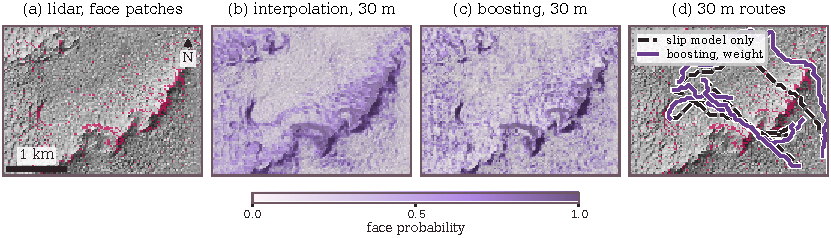
\includegraphics[width=\textwidth]{figures/fig_map.pdf}
\caption{Kelso Dunes. (a) Hillshade of the one metre lidar with face patches (plum). (b) Face probability of the calibrated interpolation layer and (c) of boosting, both on the 30\,m block mean and trained or calibrated on the other five sites. (d) Routes on the 30\,m map between six of the E1 pairs: slip model only (dashed) and boosting with the weight policy, $w=100$ (solid), over the face patches.}
\end{figure}
\begin{figure}[H]
\centering
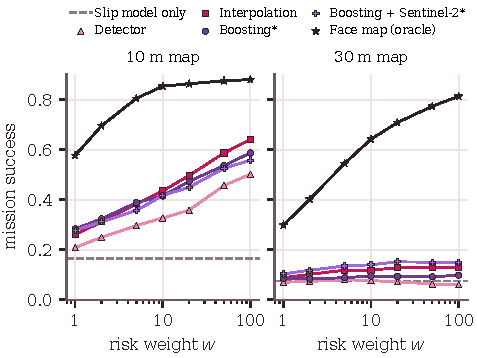
\includegraphics[width=0.62\textwidth]{figures/fig_frontier.pdf}
\caption{Mission success of the weight policy against the risk weight $w$ for each hazard layer (E1 endpoints, posterior vehicle, 600 pairs). Dashed: the slip model alone. The face map is an upper bound that needs face information from fine data. $^{*}$Trained leave one site out.}
\end{figure}

\section*{S5. Notes on the runs}
\textit{Data.} Lidar windows, projects and acquisition periods are in Table~I of the paper and in \url{results/benchmark/site_metadata.csv}. Sentinel-2 scenes: Dumont and Kelso 2024-12-20, White Sands 2020-12-19, Great Sand Dunes 2020-12-24, Algodones 2021-12-26, Little Sahara 2020-12-21; NAIP years 2021 to 2023. All crops carry SHA-256 values in \url{data/raw/extra/MANIFEST.json}.

\textit{GLO-30 alignment.} The horizontal shift that best aligns GLO-30 with the 30\,m lidar block mean is 0\,m at Dumont, 0\,m at Kelso, 11\,m at Great Sand Dunes, 11\,m at Little Sahara, 15\,m at Algodones and 31\,m at White Sands, an actively migrating gypsum dune field whose lidar is years younger than the radar acquisition.

\textit{Learned layers.} Boosting: scikit-learn histogram gradient boosting, learning rate 0.05, 300 iterations, 31 leaves; tuned version: learning rate 0.05 or 0.1, 15 or 63 leaves, 200 or 600 iterations, chosen by inner leave one site out AUC. Network: two input channels (elevation minus its $7\times7$ mean over the spacing, and the slope), four $3\times3$ convolutions of 32 channels with dilations 1, 2, 4 and 8, binary cross entropy, Adam~\cite{kingma2015adam} at 0.001, 1500 (or 6000) steps of 16 random crops with flips and quarter turns. Super resolution: the same body predicts the 5\,m lidar block mean minus the cubic spline of the 30\,m surface, L1 loss, 3000 steps of 16 crops of $96\times96$ cells. Detector: logistic model on log transformed slope, convexity, slope break and relief and their pairwise products, trained on 60\,000 synthetic straight crested dune profiles (stoss slope 6 to 20\,degrees, face 29.5 to 32.5\,degrees, height 5 to 120\,m) sampled as a DEM samples them, and applied to two dimensional grids along the steepest descent direction; this mapping has not been validated separately.

\textit{Statistics.} AUC intervals use a spatial block bootstrap with 300\,m blocks and 1000 resamples; paired differences resample the same blocks for both layers, and per site counts are also given with Bonferroni adjusted intervals (99.2\,\%) in \url{results/benchmark/stage27/A_paired_differences.csv}. The label correlogram reaches 0.1 at 30 to 870\,m, so the main 30\,m comparisons were repeated with 870\,m blocks (\url{I_larger_blocks.csv}). Planning differences carry two stage bootstrap intervals (4000 resamples of sites, then of pairs within the drawn sites), and every site level claim uses an exact sign flip test over the six per site differences.

\textit{Scoring details.} Counting a face within one post of the route (a vehicle footprint) raises the unsafe share of slip only routes at 30\,m from 92.5\,\% to 93.5\,\%; 2\,\% of the unsafe slip only routes touch faces only while descending the fall line, which some vehicles might survive; and the 28\,degree descent rule removes at most 0.05\,\% of the graph edges on the 30\,m grid, so it hardly acts there.

\textit{Spatial correlation.} The labels are spatially correlated over 30 to 870\,m (the largest at Dumont, whose window holds rocky hills); with 870\,m blocks the per site intervals of slope and the detector still lie below interpolation at all six sites.

\textit{Runtime.} On one core of a cloud x86 machine, assessing a 10\,km$^2$ window and planning 100 routes on it take 0.2 and 0.2\,s at 30\,m.

\section*{S6. Degraded face maps and post hoc checks}
\begin{table}[H]
\caption{Mission success (\%) at the operating point chosen on the other five sites (gate threshold or weight), 100 pairs per site, posterior vehicle. E1: endpoints chosen with the truth; E2: chosen from the coarse map only. $^{\dagger}$Two stage bootstrap interval of the gain over the slip model entirely above zero (not corrected for the number of cells). Lower part, a second protocol: face maps degraded as registered, weight policy at a fixed $w=5$. $\cdot$ not run. $^{*}$Trained leave one site out.}
\label{tab:planning_s}
\centering\scriptsize
\setlength{\tabcolsep}{3pt}
\begin{tabular}{@{}lccccc@{}}
\toprule
 & \multicolumn{2}{c}{I10} & \multicolumn{2}{c}{I30} & G30 \\
Layer & E1 & E2 & E1 & E2 & E1 \\
\midrule
Slip model only & 17 & 9 & 8 & 3 & 6 \\
Slope & 35$^{\dagger}$ & 28$^{\dagger}$ & 6 & 3 & 6 \\
Interpolation & 64$^{\dagger}$ & 53$^{\dagger}$ & 13$^{\dagger}$ & 5 & 7 \\
Detector & 50$^{\dagger}$ & 33$^{\dagger}$ & 7 & 4 & 5 \\
Boosting$^{*}$ & 59$^{\dagger}$ & 47$^{\dagger}$ & 9 & 4 & 7 \\
Network$^{*}$ & 51$^{\dagger}$ & 40$^{\dagger}$ & 6 & 3 & 7 \\
Boosting + Sentinel-2$^{*}$ & 56$^{\dagger}$ & 46$^{\dagger}$ & 13$^{\dagger}$ & 7$^{\dagger}$ & $\cdot$ \\
Face map (oracle) & 84$^{\dagger}$ & 80$^{\dagger}$ & 81$^{\dagger}$ & 68$^{\dagger}$ & 80$^{\dagger}$ \\
\midrule
Face map, $w=5$ & 81 & 71 & 55 & 40 & $\cdot$ \\
Face map 5\,m off & 67 & 56 & 50 & 39 & $\cdot$ \\
Face map 10\,m off & 36 & 26 & 43 & 32 & $\cdot$ \\
Face map 30\,m off & 19 & 10 & 11 & 5 & $\cdot$ \\
Face map from 2\,m survey & 29 & 19 & 23 & 14 & $\cdot$ \\
Face map from 5\,m survey & 17 & 9 & 8 & 4 & $\cdot$ \\
\bottomrule
\end{tabular}
\end{table}

These checks were decided after the main results were known and are post hoc (stages 29 and 30 of the log).

\textit{Larger faces by post count.} Scored only on face patches of at least 300 posts, the slip model alone succeeds on 30\,\% of the 30\,m routes and interpolation on 43\,\%; on 10\,m maps the values are 39\,\% and 93\,\%. Without Dumont, whose window holds rocky hills, the 30\,m values are 31\,\% and 47\,\%.

\textit{Other face rules.} A hysteresis rule (posts of 25\,degrees or more, groups of at least 10 posts holding one post of 30\,degrees or more) gives 7\,931 patches against 14\,638 with the registered rule, and a rule that closes gaps of one post before grouping gives 11\,783. Mission success on I30 (E1) scored against these rules: slip model alone 6\,\% and 8\,\%, interpolation 9\,\% and 12\,\%.

\textit{Exposure.} Metres on face patches per km of route on I30 (E1): slip model alone 32.9, interpolation 11.4, boosting with Sentinel-2 8.3, face map oracle 2.1; on I10 12.6, 1.0 and 0.3.

\textit{Survey face maps.} The face maps from simulated surveys fail because the 28\,degree rule misses faces on a coarser grid: the 2\,m survey marks 59\,\% to 91\,\% of the face patch posts, depending on the site, and the 5\,m survey 8\,\% to 78\,\%, below 60\,\% at four sites. A survey face map needs a threshold calibrated for its own spacing.

\textit{GLO-30 alignment and migration.} At Dumont and Kelso, where GLO-30 matches the lidar without shift, interpolation of GLO-30 on its own grid reaches an AUC of 0.85, against 0.62 at the other four sites. Applying the best shift at every site changes the mean AUC of interpolation only from 0.70 to 0.70, and planning with it from 7\,\% to 6\,\% (slip model alone 6\,\% and 6\,\%). The contrast between the two groups of sites therefore probably reflects how hard the sites are rather than misregistration.

\textit{Extended weight grid.} With the weight policy over $w$ up to 1000, held out success on I10 (E1) is 66\,\% for interpolation (registered grid 64\,\%), 65\,\% for boosting (59\,\%), and on I30 83\,\% for the oracle (81\,\%); no computable layer on I30 changes by more than two points.

\textit{Finer and learned inputs.} On 5\,m block means with weights up to 1000, interpolation reaches 86\,\% against 34\,\% for the slip model alone and the oracle 93\,\%. On 30\,m maps the best layers from elevation alone add little: super resolution +5 points (interval +2 to +8) and the network trained for 6000 steps +2.

\textit{Displaced face maps.} With the weight chosen on the other five sites from a grid up to 1000, where the oracle itself reaches 84\,\%, the face map gives 75\,\% displaced by 5\,m, 61\,\% by 10\,m and 11\,\% by 30\,m.

\begin{table}[H]
\caption{Registered closed loop with an idealised sensor (radius $R$), 20 pairs per site, posterior vehicle, sensing every face within the radius: success (\%; goal reached, no face contact) and replans per pair (Rp), E1 endpoints unless marked E2. Main runs $R=20$\,m; I30 also with $R=10$ and 30\,m.}
\label{tab:closedloop_ideal}
\centering\scriptsize
\setlength{\tabcolsep}{2.4pt}
\begin{tabular}{@{}lccccccc@{}}
\toprule
 & \multicolumn{2}{c}{I10, $R$ 20} & \multicolumn{2}{c}{I30, $R$ 20} & \multicolumn{3}{c}{I30, S} \\
Prior layer & S & Rp & S & Rp & E2 & $R$ 10 & $R$ 30 \\
\midrule
Slip model only & 78 & 11 & 80 & 29 & 67 & 76 & 83 \\
Detector & 81 & 5 & 85 & 25 & 73 & 82 & 85 \\
Interpolation & 80 & 4 & 82 & 20 & 71 & 81 & 87 \\
Boosting$^{*}$ & 80 & 4 & 84 & 21 & 71 & 81 & 88 \\
Face map & 80 & 1 & 85 & 8 & 75 & 83 & 86 \\
\bottomrule
\end{tabular}
\end{table}

\end{document}
